\documentclass{article}
\title{CSCD350, Holiday Mailer: Software Requirements Specification}
\author{Steve Berg, Zach Lesperance, Tim Lynch, Steven Mather}
\date{\today}

\usepackage{graphicx}
\usepackage{float}
\usepackage[margin=1in]{geometry}
\setlength{\parindent}{0pt}

\begin{document}

\maketitle{}
\pagebreak

\section{Introduction}
%This section provides an overview of the entire requirement document. This document describes all data, functional and behavioral requirements for software.

\subsection{Goals and objectives}
To build a program that stores addresses of friends and relatives and allows the user to send a `Holiday Email' to people of her/his choice.

%\subsection{Statement of scope}
%A description of the software is presented. Major inputs, processing functionality and outputs are described without regard to implementation detail.

\subsection{Software context}
%The software is placed in a business or product line context. Strategic issues relevant to context are discussed. The intent is for the reader to understand the 'big picture'.
Consumer grade product that is intuitive for use by the average computer user. The software handles their `Holiday Letters' for them electronically.

\subsection{Major constraints}
%Any business or product line constraints that will impact the manner in which the software is to be specified, designed, implemented or tested are noted here.
The software will need to be able to run minimally on a consumer grade machine so as to not noticeably impact performance.
Web connection while running to allow access to the external e-mail servers.

%\section{Usage scenario}
%This section provides a usage scenario for the software. It organized information collected during requirements elicitation into use-cases.

%\subsection{User profiles}
%The profiles of all user categories are described here.


\subsection{Use-cases}
%All use-cases for the software are presented.
\subsubsection*{Use case Add new person to database}
Actor user \\
Basic choose to enter new person, enter first name, enter last name, enter address, enter if and email was sent, submit to database \\

\subsubsection*{Use case Remove person from database}
Actor user \\
Basic choose to remove, choose who to remove, make sure, remove \\
 
\subsubsection*{Use case Display entries by last name}
Actor user \\
Basic choose to display, choose to display by last name, display \\
 
\subsubsection*{Use case Display entries by first name}
Actor user \\
Basic choose to display, choose to display by first name, display \\
 
\subsubsection*{Use case Display entries by last received date}
Actor user \\
Basic choose to display, choose to display by last received date, display \\

\subsubsection*{Use case Display entries with last name with certain letter}
Actor user \\
Basic choose to display, choose to display by certain letters, display \\
 
\subsubsection*{Use case send email to everyone}
Actor user \\
Basic choose to send email to everyone, pick holiday email to send, send \\
 
\subsubsection*{Use case send email to everyone who has sent one}
Actor user \\
Basic choose to send email to everyone who has sent you one, pick holiday email to send, send \\
 
\subsubsection*{Use case send email to specific people}
Actor user \\
Basic choose to send email to specific people, pick people, pick holiday email to send, send \\

\subsection*{Use Case Diagram}
\begin{figure}[H]
\centering
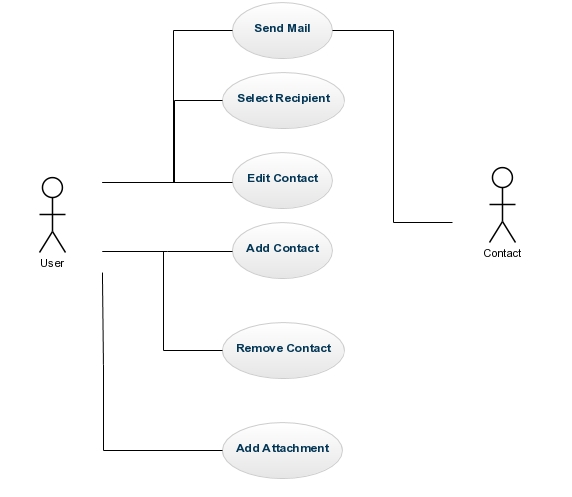
\includegraphics[width=110mm]{img/finalDiagrams/UseCaseDiagram.jpg}
\caption{Use Case Diagram \label{useCase}}
\end{figure}


%\subsection{Special usage considerations}
%Special requirements associated with the use of the software are presented.

\section{Data Model and Description}
%This section describes information domain for the software
For this project, we will be using SQLite technology for our data object interactions.

\subsection{Data Description}
%Data objects that will be managed/manipulated by the software are described in this section.

\subsubsection{Data objects}
%Data objects and their major attributes are described.
\textbf{Name}: contacts \\
\textbf{Description}: A table that stores all of the user's contacts and their information \\
\textbf{Fields:}
\begin{itemize}
\item email (varchar(50)): The contact's email address
\item firstName (varchar(50)): The contact's first name
\item lastName (varchar(50)): The contact's surname
\item lastReceivedYear (int): The year that the contact last sent a holiday letter to the user
\end{itemize}

%\subsubsection{Relationships}
%Relationships among data objects are described using an ERD- like form. No attempt is made to provide detail at this stage.

\subsubsection{Complete data model}
%An ERD for the software is developed
\begin{figure}[H]
\centering
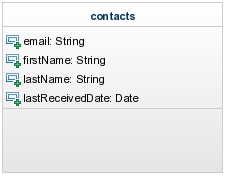
\includegraphics[width=90mm]{img/db_erd.jpg}
\caption{Entity-Relation Diagram for our Data Model \label{db_erd}}
\end{figure}

%\subsubsection{Data dictionary}
%A reference to the data dictionary is provided. The dictionary is maintained in electronic form.

\section{Functional Model and Description}
%A description of each major software function, along with data flow or class hierarchy (OO) is presented.
The Client class is the main anchor for the program. \\
It contains references to two objects that handle all input from the user and all output to the user. \\
The client will also contain the methods needed to delegate work to the proper objects, i.e. contact creation, contact modification, contact deletion, display. \\

The DBAccess object will be used for all interaction with the database. \\
The MailControl object track any additions and removals and save them to the database using DBAccess. \\
The contact class is an object that represents tuples in the database. \\
The userOut object handles the interactions the program has with the user. \\
\begin{figure}[H]
\centering
%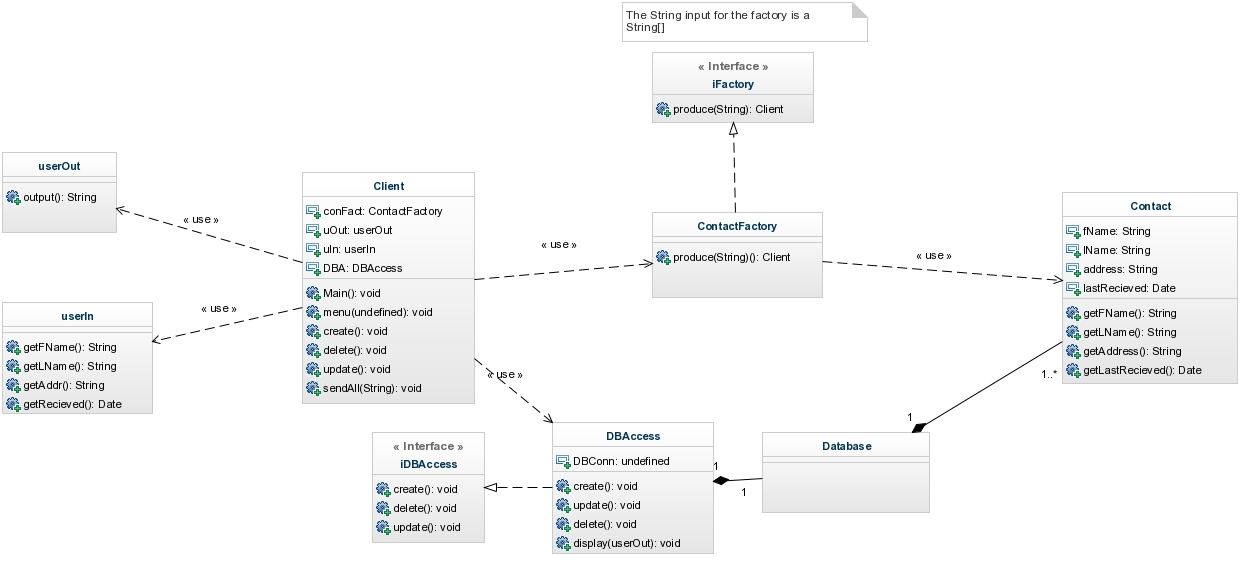
\includegraphics[width=170mm]{img/UML.jpg}
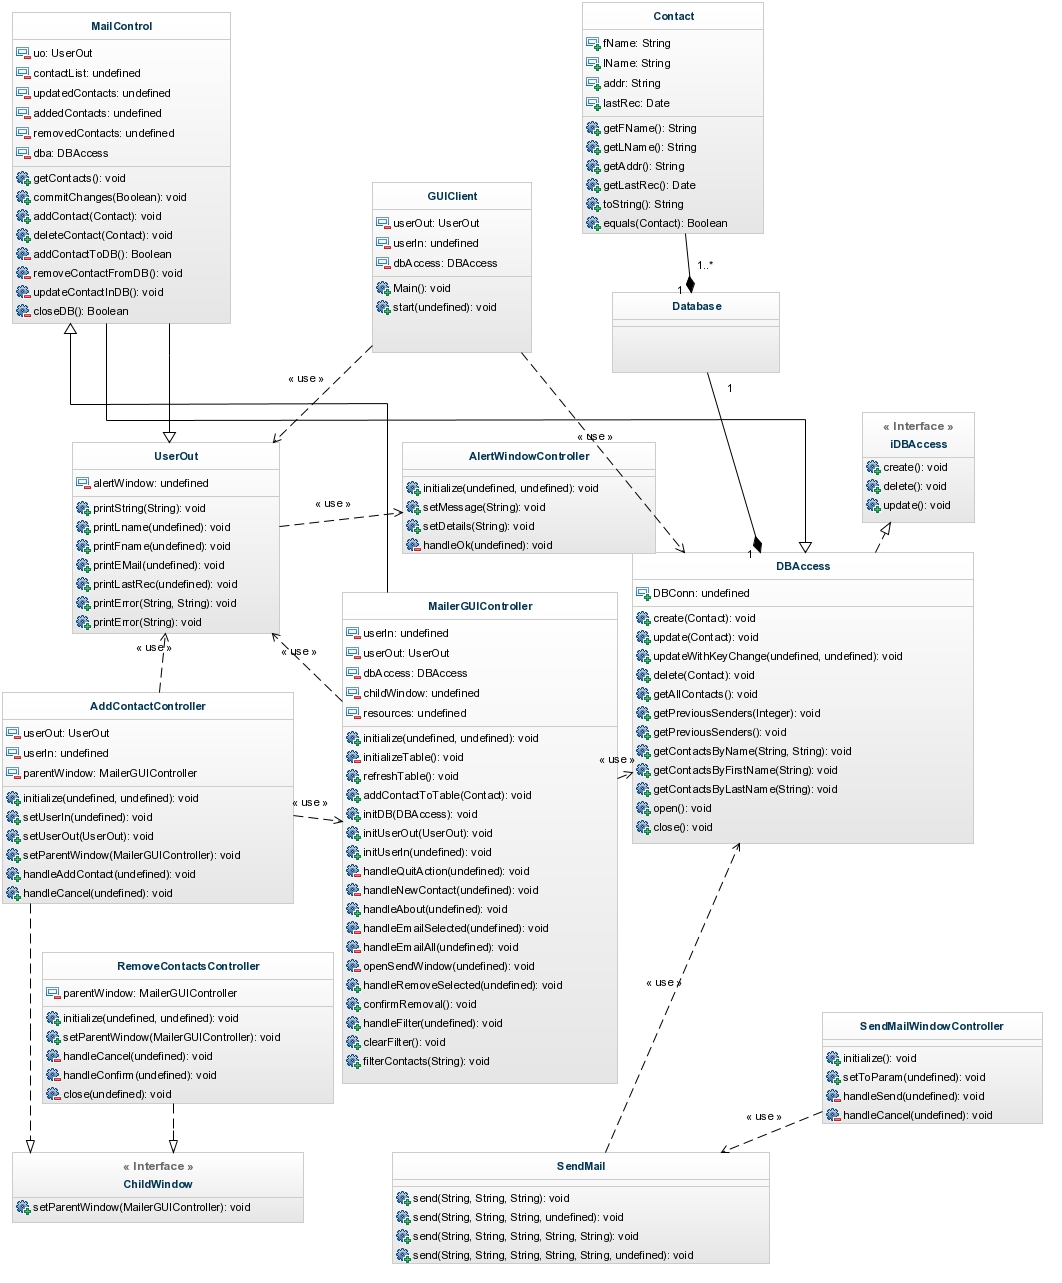
\includegraphics[width=180mm]{img/finalDiagrams/ClassDiagram.jpg}
\caption{UML Class Diagram of the Software \label{UML}}
\end{figure}

%\subsection{Description for Function n}
%A detailed description of each software function is presented. Section 4.1 is repeated for each of n functions.

%\subsubsection{Processing narrative (PSPEC) for function n}
%A processing narrative for function n is presented.

%\subsubsection{Function n flow diagram}
%A diagram showing the flow of information through the function and the transformation it undergoes is presented.

%\subsubsection{Function n interface description}
%A detailed description of the input and output interfaces for the function is presented.

%\subsubsection{Function n transforms}
%A detailed description for each transform (subfunction) for function n is presented. Section 4.1.4 is repeated for each of k transforms.

%Transform k description (processing narrative, PSPEC)

%Transform k interface description

%Transform k lower level flow diagrams

%Transform k interface description

%\subsubsection{Performance Issues}
%Special performance required for the subsystem is specified.

%\subsubsection{Design Constraints}
%Any design constraints that will impact the subsystem are noted.

\subsection{Software Interface Description}
%The software interface(s)to the outside world is(are) described.

%\subsubsection{External machine interfaces}
%Interfaces to other machines (computers or devices) are described.

%\subsubsection{External system interfaces}
%Interfaces to other systems, products or networks are described.

\subsubsection{Human interface}
%An overview of any human interfaces to be designed for the software is presented.
A command line menu driven interface will initially be built and if time permits and we make all the properties that we want, a graphical user interface will be build.

%\subsection{Control flow description}
%The control flow for the system is presented with reference to Section 5.0 of this document.

\section{Behavioral Model and Description}
A description of the behavior of the software is presented.

%\subsection{Description for software behavior}
%A detailed description of major events and states is presented in this section.

%\subsubsection{Events}
%A listing of events (control, items) that will cause behavioral change within the system is presented.

\subsubsection{States}

State: IDLE \\
Description: Program window is open and waiting for user interaction. \\

State: Add Contact \\
Description: User has requested to add a contact, the add contact form appears, the user fills it out and submits it, returning to IDLE. \\

State: Select Contact \\
Description: User has selected one or more contacts from the table of available contacts. \\

State: Remove Contact \\
Description: User has selected to remove contact. User is alerted that this action cannot be undone. User can accept or cancel the request, either returning the program to IDLE. \\

State: Add Attachment \\
Description: User has selected one or more contacts to receive an email and has chosen to add an attachment. User can select a file on their local file system to attach. \\

State: Send Mail \\
Description: User has chosen to send emails to one or more contacts. The system sends the mail and returns to IDLE. \\


\subsection{State Transition Diagrams}
\begin{figure}[H]
\centering
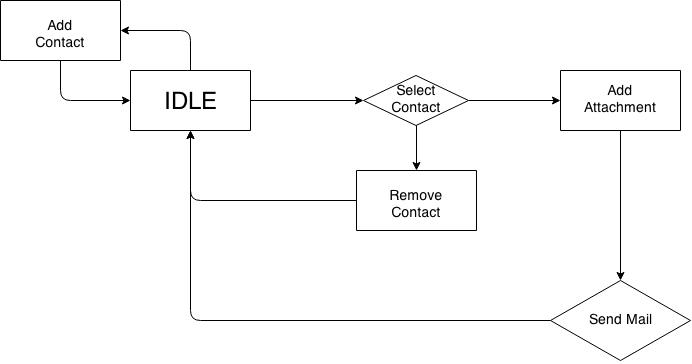
\includegraphics[width=140mm]{img/finalDiagrams/StateDiagram.jpg}
\caption{UML State Diagram of the Software \label{State}}
\end{figure}

\subsection*{Sequence Diagram}
\begin{figure}[H]
\centering
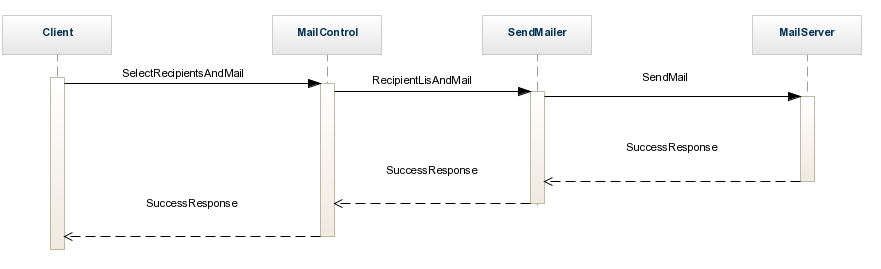
\includegraphics[width=150mm]{img/finalDiagrams/SequenceDiagram.jpg}
\caption{Sequence Diagram of the Software \label{sequence}}
\end{figure}



%\subsection{Control specification (CSPEC)}
%Depict the manner in which control is managed by the software.

%\section{Restrictions, Limitations, and Constraints}
%Special issues which impact the specification, design, or implementation of the software are noted here.

\section{Validation Criteria}
%The approach to software validation is described.

\subsection{Classes of tests}
%The types of tests to be conducted are specified, including as much detail as is possible at this stage. Emphasis here is on black- box testing.
We will be running JUnit tests against each iteration of our code to make sure that our program stays consistent. \\

JUnit will be testing:
\begin{itemize}
\item All CRUD (Create Update Delete) methods, database interation, data validation, etc methods.
\item The ability to send mail
\item User input functions
\end{itemize}

%\subsection{Expected software response}
%The expected results from testing are specified.

%\subsection{Performance bounds}
%Special performance requirements are specified. 

%\section{Appendices}
%Presents information that supplements the Requirements Specification

%\subsection{System traceability matrix}
%A matrix that traces stated software requirements back to the system specification.

%\subsection{Product Strategies}
%If the specification is developed for a product, a description of relevant product strategy is presented here.

%\subsection{Analysis metrics to be used}
%A description of all analysis metrics to be used during the analysis activity is noted here.

%\subsection{Supplementary information (as required)}

\end{document}
